\documentclass[11pt]{article}

\usepackage{epsfig}
\usepackage{amsfonts}
\usepackage{amssymb}
\usepackage{amstext}
\usepackage{amsmath}
\usepackage{xspace}
\usepackage{theorem}
\usepackage{graphicx}
\usepackage{tikz}
\usepackage{pgfplots}

% \usepackage{layout}% if you want to see the layout parameters
% and now use \layout command in the body

% This is the stuff for normal spacing
\makeatletter
 \setlength{\textwidth}{6in}
 \setlength{\oddsidemargin}{0in}
 \setlength{\evensidemargin}{0.5in}
 \setlength{\topmargin}{0in}
 \setlength{\textheight}{9in}
 \setlength{\headheight}{0pt}
 \setlength{\headsep}{0pt}
 \setlength{\marginparwidth}{59pt}

 \setlength{\parindent}{0pt}
 \setlength{\parskip}{5pt plus 1pt}
 \setlength{\theorempreskipamount}{5pt plus 1pt}
 \setlength{\theorempostskipamount}{0pt}
 \setlength{\abovedisplayskip}{8pt plus 3pt minus 6pt}


\newenvironment{proof}{{\bf Proof:  }}{\hfill\rule{2mm}{2mm}}
\newenvironment{proofof}[1]{{\bf Proof of #1:  }}{\hfill\rule{2mm}{2mm}}
\newenvironment{proofofnobox}[1]{{\bf#1:  }}{}
\newenvironment{example}{{\bf Example:  }}{\hfill\rule{2mm}{2mm}}


\newtheorem{theorem}{Theorem}
\newtheorem{lemma}[theorem]{Lemma}
\newtheorem{proposition}[theorem]{Proposition}
\newtheorem{claim}[theorem]{Claim}
\newtheorem{corollary}[theorem]{Corollary}
\newtheorem{definition}[theorem]{Definition}

% math notation
\newcommand{\R}{\ensuremath{\mathbb R}}
\newcommand{\Z}{\ensuremath{\mathbb Z}}
\newcommand{\N}{\ensuremath{\mathbb N}}
\newcommand{\F}{\ensuremath{\mathbb F}}
\newcommand{\C}{\ensuremath{\mathbb C}}

\newcommand{\size}[1]{\ensuremath{\left|#1\right|}}
\newcommand{\ceil}[1]{\ensuremath{\left\lceil#1\right\rceil}}
\newcommand{\floor}[1]{\ensuremath{\left\lfloor#1\right\rfloor}}


% anupam's abbreviations
\newcommand{\mnote}[1]{\normalmarginpar \marginpar{\tiny #1}}


% vectors
\renewcommand{\vec}[1]{\ensuremath{\mathbf{#1}}}

\newenvironment{sol}
    {\emph{Solution:}
    }


%%%%%%%%%%%%%%%%%%%%%%%%%%%%%%%%%%%%%%%%%%%%%%%%%%%%%%%%%%%%%%%%%%%%%%%%%%%
% Document begins here %%%%%%%%%%%%%%%%%%%%%%%%%%%%%%%%%%%%%%%%%%%%%%%%%%%%
%%%%%%%%%%%%%%%%%%%%%%%%%%%%%%%%%%%%%%%%%%%%%%%%%%%%%%%%%%%%%%%%%%%%%%%%%%%


\newcommand{\headings}{
\large{\textbf{YOUR NAME GOES HERE \hfill 21-241 Fall 2019}\\
\textbf{Homework 7 \hfill Due Friday, October 18}}\\
\rule[0.1in]{\textwidth}{0.01in}
%\thispagestyle{empty}
}

\pagestyle{empty}

\begin{document}

\headings




\begin{enumerate}
\section*{Required Problems}



\item (Strang 5.1.8) Prove that every orthogonal matrix ($Q^TQ=I$) has determinant 1 or -1.

\begin{enumerate}
\item Use the product rule $\det AB = \det A \det B$ and the transpose rule $\det Q = \det Q^T$.
\item Use only the product rule.  If $|\det Q|>1$, then $\det Q^n = (\det Q)^n$ blows up.  How do you know this can't happen to $Q^n$?
\end{enumerate}

 \begin{sol}
Write your solution here.
\end{sol}
\clearpage

\item (Strang 5.1.10) If the entries in every row of $A$ add to zero, solve $A\vec{x} = \vec{0}$ to prove $\det A = 0$. If those entries add to one, show that $\det(A-I) = 0$. Does this mean $\det A = 1$?

 \begin{sol}
Write your solution here.
\end{sol}
\clearpage

\item (Strang 5.1.23) From $A = \begin{bmatrix} 4 & 1 \\ 2 & 3 \end{bmatrix}$, find $A^2$ and $A^{-1}$ and $A-\lambda I$ and their determinants.  Which two numbers $\lambda$ lead to $\det (A- \lambda I) = 0$?


 \begin{sol}
Write your solution here.
\end{sol}
\clearpage

\item Strang (5.2.4) Find two ways to choose nonzeros from four different rows and columns:

\[A= \begin{bmatrix} 1 & 0 & 0 & 1 \\ 0 & 1 & 1 & 1 \\ 1 & 1 & 0 & 1 \\ 1 & 0 & 0 & 1 \end{bmatrix} \quad 
B = \begin{bmatrix} 1 & 0 & 0 & 2 \\ 0 & 3 & 4 & 5 \\ 5 & 4 & 0 & 3 \\ 2 & 0 & 0 & 1 \end{bmatrix}\]
($B$ has the same zeros as $A$). Is $\det A$ equal to $1+1$ or $1-1$ or $-1-1$?  What is $\det B$?

 \begin{sol}
Write your solution here.
\end{sol}
\clearpage

\item (From Strang 5.2.12) Find the cofactor matrix $C$ and multiply $A$ times $C^T$. Compare $C^T$ with $A^{-1}$:

\[A= \begin{bmatrix} 2 & -1 & 0 \\ -1 & 2 & -1 \\  0 & -1 & 2 \end{bmatrix} \quad 
A^{-1} = \frac{1}{4} \begin{bmatrix} 3 & 2 & 1 \\ 2 & 4 & 2 \\ 1 & 2 & 3 \end{bmatrix}\]


 \begin{sol}
Write your solution here.
\end{sol}
\clearpage


\item\label{rotref}



\begin{enumerate}
\item The rotation matrix $R_\theta = \begin{bmatrix} \cos \theta & -\sin \theta \\ \sin \theta & \cos \theta\end{bmatrix}$ rotates each point in the the plane counterclockwise around the origin by angle $\theta$.

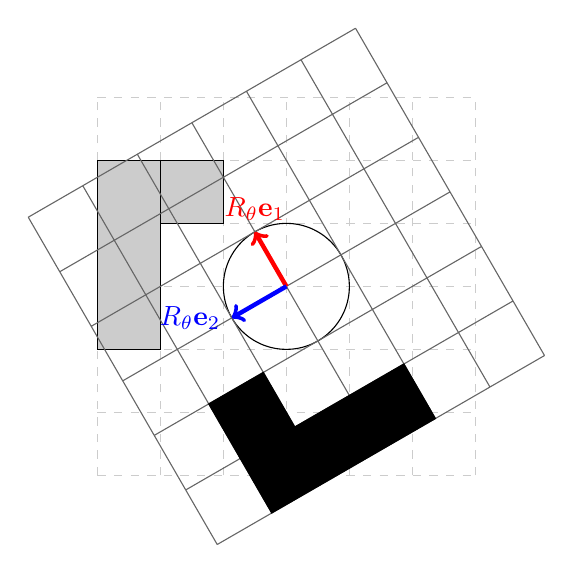
\begin{tikzpicture}[scale=.8]
    \draw [very thin,gray!40,dashed] (-3,-3) grid (3,3);
           \draw[fill=gray!40] (-3,-1) rectangle (-2,2);
       \draw[fill=gray!40] (-2,1) rectangle (-1,2);
       \draw (0,0) circle (1cm);
    %Specify the transformation matrix and the center point
    \pgftransformcm{-.5}{.866}{-.866}{-.5}{\pgfpoint{0}{0}}
    \draw [black!60] (-3,-3) grid (3,3);
    \draw [ultra thick,red,->] (0,0)  -- (1,0) node [above] {$R_\theta \vec{e}_1$}; 
    \draw [ultra thick,blue,->] (0,0) -- (0,1) node [left] {$R_\theta \vec{e}_2$};
        \draw[fill=black] (-3,-1) rectangle (-2,2);
     \draw[fill=black] (-2,1) rectangle (-1,2);
\end{tikzpicture}



\begin{itemize}
\item What is $\det R_\theta$?
\item How much is area scaled by $R_\theta$?
\item Does $R_\theta$ reverse orientation?
\item Find the inverse of $R_\theta$.
\item Verify that $R_\theta$ is an orthogonal matrix.
\item Where is the point $(7,3)$ mapped by $R_{3\pi/4}$?
\end{itemize}
\item The reflection matrix $r_\theta  = \begin{bmatrix} \cos 2\theta & \sin 2\theta \\ \sin 2\theta & -\cos 2\theta\end{bmatrix}$ reflects each point in the plane over the line making angle $\theta$ with the $x$-axis.

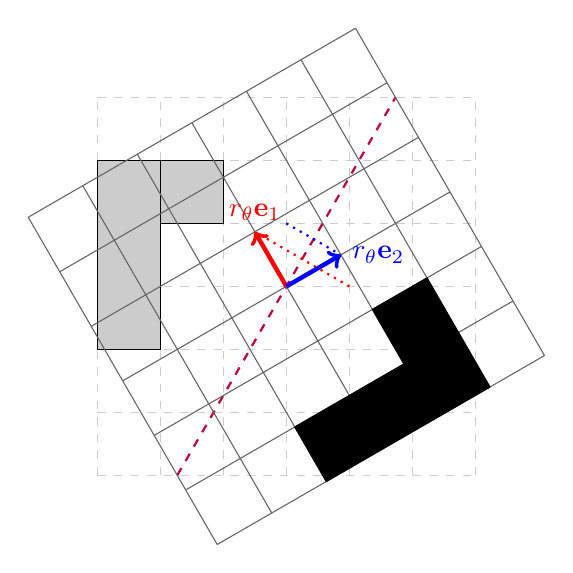
\begin{tikzpicture}[scale=.8]
    \draw [very thin,gray!40,dashed] (-3,-3) grid (3,3);
           \draw[fill=gray!40] (-3,-1) rectangle (-2,2);
       \draw[fill=gray!40] (-2,1) rectangle (-1,2);
       \draw[thick, dashed, purple] (-1.732,-3) -- (1.732,3);
       \draw[thick, blue, dotted] (0,1) -- (.866,.5);
        \draw[thick, red, dotted] (1,0) -- (-.5,.866);
    %Specify the transformation matrix and the center point
    \pgftransformcm{-.5}{.866}{.866}{.5}{\pgfpoint{0}{0}}
    \draw [black!60] (-3,-3) grid (3,3);
    \draw [ultra thick,red,->] (0,0)  -- (1,0) node [above] {$r_\theta \vec{e}_1$}; 
    \draw [ultra thick,blue,->] (0,0) -- (0,1) node [right] {$r_\theta \vec{e}_2$};
        \draw[fill=black] (-3,-1) rectangle (-2,2);
     \draw[fill=black] (-2,1) rectangle (-1,2);
\end{tikzpicture}
\begin{itemize}
\item What is $\det r_\theta$?
\item How much is area scaled by $r_\theta$?
\item Does $r_\theta$ reverse orientation?
\item Find the inverse of $r_\theta$.
\item Verify that $r_\theta$ is an orthogonal matrix.
\item Where is the point $(7,3)$ mapped by $r_{3\pi/4}$?
\end{itemize}
\end{enumerate}

 \begin{sol}
Write your solution here.
\end{sol}
\clearpage

\item Each part below shows the image of the grid where $-3 \le x \le 3$ and $-3 \le y \le 3$ after being transformed by a $2 \times 2$ matrix $A$. The original grid is shown lightly in the background. The gray area is mapped to the black area.. For each image,
\begin{itemize}
\item Find the matrix $A$.
\item Find the determinant of $A$.
\item Find the area of one parallelogram in the transformed grid.
\item State whether $A$ preserves or reverses orientation.
\end{itemize}

\begin{enumerate}
\item \

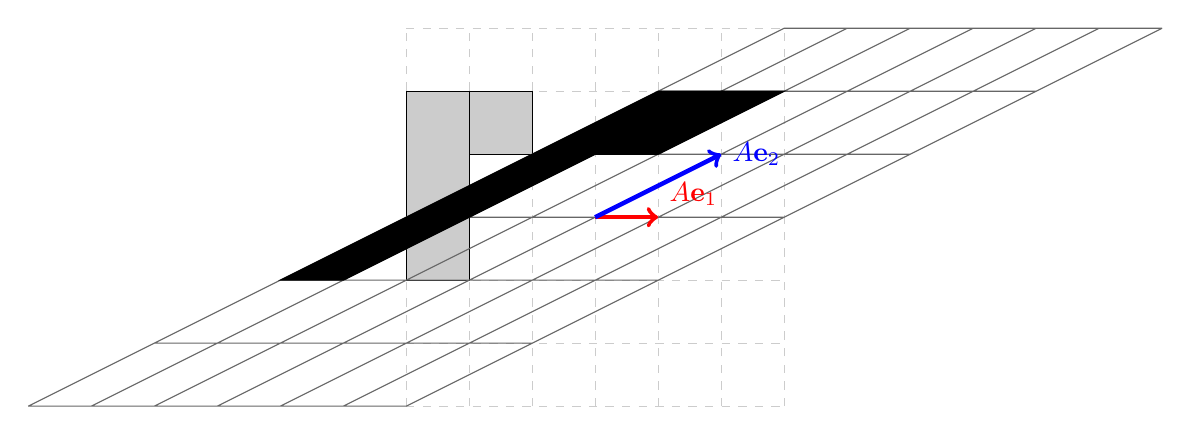
\begin{tikzpicture}[scale=.8]
    \draw [very thin,gray!40,dashed] (-3,-3) grid (3,3);
       \draw[fill=gray!40] (-3,-1) rectangle (-2,2);
       \draw[fill=gray!40] (-2,1) rectangle (-1,2);
    %Specify the transformation matrix and the center point
    \pgftransformcm{1}{0}{2}{1}{\pgfpoint{0}{0}}
    \draw [black!60] (-3,-3) grid (3,3);
    \draw [ultra thick,red,->] (0,0)  -- (1,0) node [above right] {$A\vec{e}_1$}; 
    \draw [ultra thick,blue,->] (0,0) -- (0,1) node [right] {$A\vec{e}_2$};
    \draw[fill=black] (-3,-1) rectangle (-2,2);
     \draw[fill=black] (-2,1) rectangle (-1,2);
\end{tikzpicture}

\item \

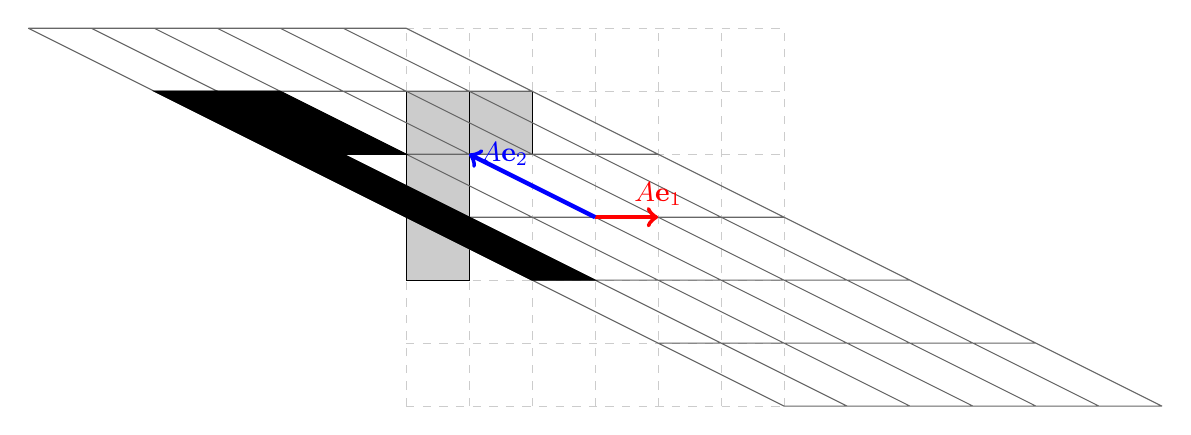
\begin{tikzpicture}[scale=.8]
    \draw [very thin,gray!40,dashed] (-3,-3) grid (3,3);
           \draw[fill=gray!40] (-3,-1) rectangle (-2,2);
       \draw[fill=gray!40] (-2,1) rectangle (-1,2);
    %Specify the transformation matrix and the center point
    \pgftransformcm{1}{0}{-2}{1}{\pgfpoint{0}{0}}
    \draw [black!60] (-3,-3) grid (3,3);
    \draw [ultra thick,red,->] (0,0)  -- (1,0) node [above] {$A\vec{e}_1$}; 
    \draw [ultra thick,blue,->] (0,0) -- (0,1) node [right] {$A\vec{e}_2$};
        \draw[fill=black] (-3,-1) rectangle (-2,2);
     \draw[fill=black] (-2,1) rectangle (-1,2);
\end{tikzpicture}

\item \

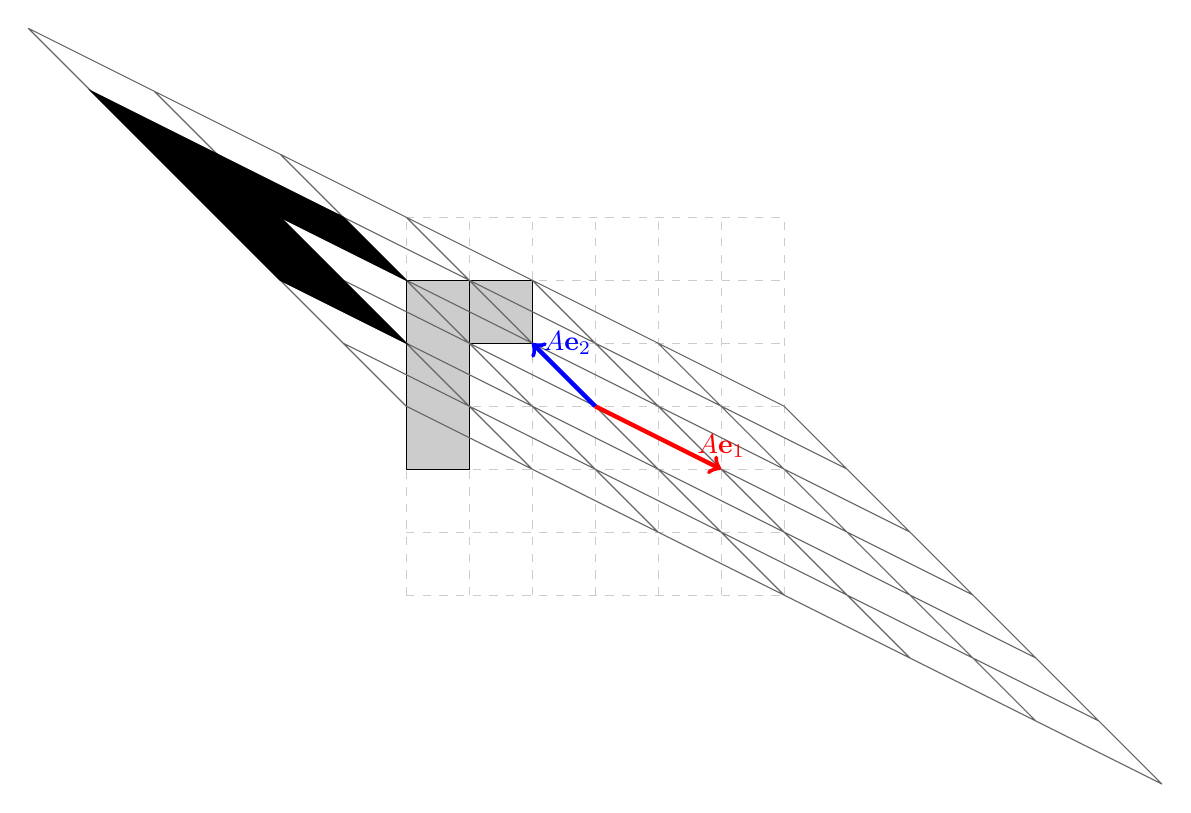
\begin{tikzpicture}[scale=.8]
    \draw [very thin,gray!40,dashed] (-3,-3) grid (3,3);
           \draw[fill=gray!40] (-3,-1) rectangle (-2,2);
       \draw[fill=gray!40] (-2,1) rectangle (-1,2);
    %Specify the transformation matrix and the center point
    \pgftransformcm{2}{-1}{-1}{1}{\pgfpoint{0}{0}}
    \draw [black!60] (-3,-3) grid (3,3);
    \draw [ultra thick,red,->] (0,0)  -- (1,0) node [above] {$A\vec{e}_1$}; 
    \draw [ultra thick,blue,->] (0,0) -- (0,1) node [right] {$A\vec{e}_2$};
        \draw[fill=black] (-3,-1) rectangle (-2,2);
     \draw[fill=black] (-2,1) rectangle (-1,2);
\end{tikzpicture}
\item \

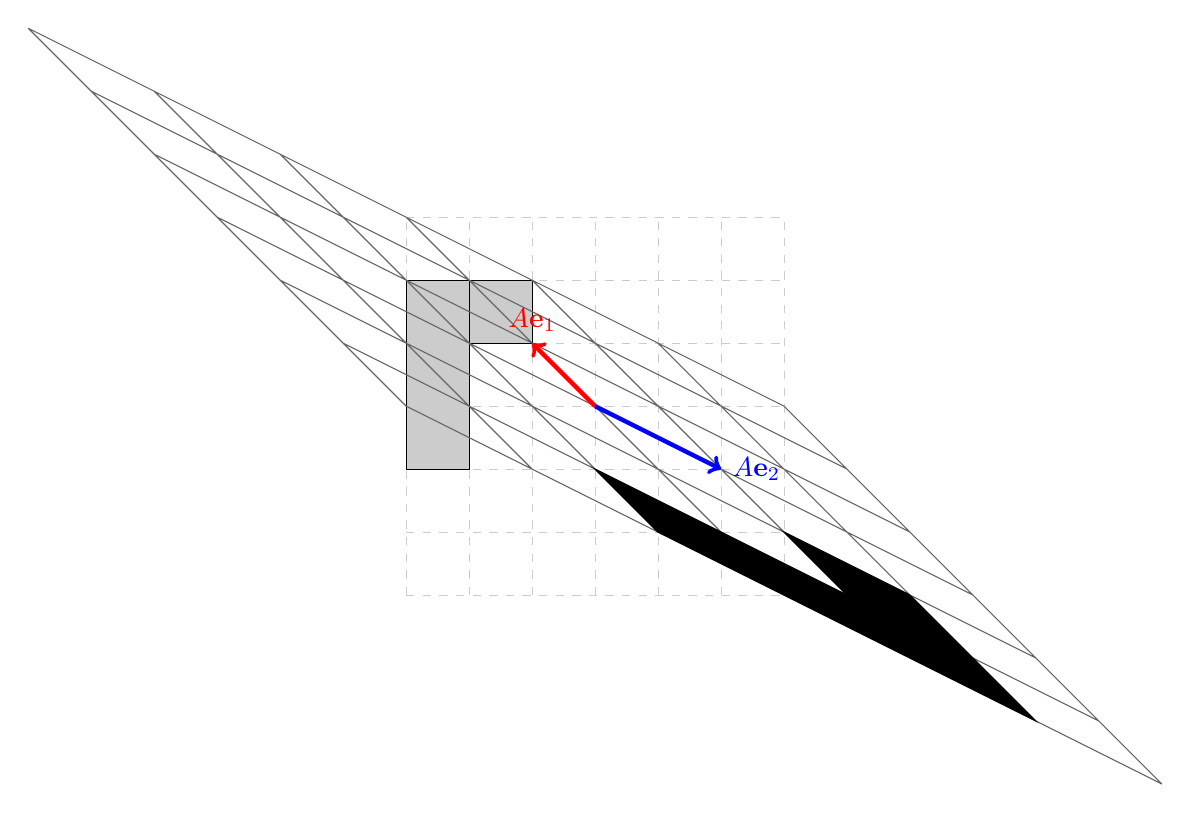
\begin{tikzpicture}[scale=.8]
    \draw [very thin,gray!40,dashed] (-3,-3) grid (3,3);
           \draw[fill=gray!40] (-3,-1) rectangle (-2,2);
       \draw[fill=gray!40] (-2,1) rectangle (-1,2);
    %Specify the transformation matrix and the center point
    \pgftransformcm{-1}{1}{2}{-1}{\pgfpoint{0}{0}}
    \draw [black!60] (-3,-3) grid (3,3);
    \draw [ultra thick,red,->] (0,0)  -- (1,0) node [above] {$A\vec{e}_1$}; 
    \draw [ultra thick,blue,->] (0,0) -- (0,1) node [right] {$A\vec{e}_2$};
        \draw[fill=black] (-3,-1) rectangle (-2,2);
     \draw[fill=black] (-2,1) rectangle (-1,2);
\end{tikzpicture}

\item \

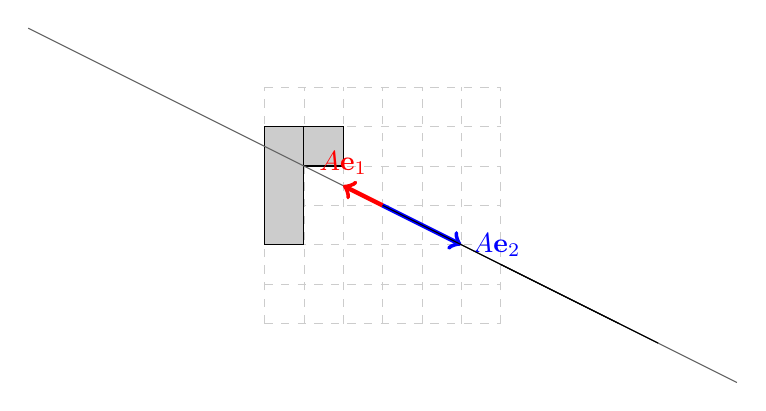
\begin{tikzpicture}[scale=.5]
    \draw [very thin,gray!40,dashed] (-3,-3) grid (3,3);
           \draw[fill=gray!40] (-3,-1) rectangle (-2,2);
       \draw[fill=gray!40] (-2,1) rectangle (-1,2);
    %Specify the transformation matrix and the center point
    \pgftransformcm{-1}{.5}{2}{-1}{\pgfpoint{0}{0}}
    \draw [black!60] (-3,-3) grid (3,3);
    \draw [ultra thick,red,->] (0,0)  -- (1,0) node [above] {$A\vec{e}_1$}; 
    \draw [ultra thick,blue,->] (0,0) -- (0,1) node [right] {$A\vec{e}_2$};
        \draw[fill=black] (-3,-1) rectangle (-2,2);
     \draw[fill=black] (-2,1) rectangle (-1,2);
\end{tikzpicture}

\item \

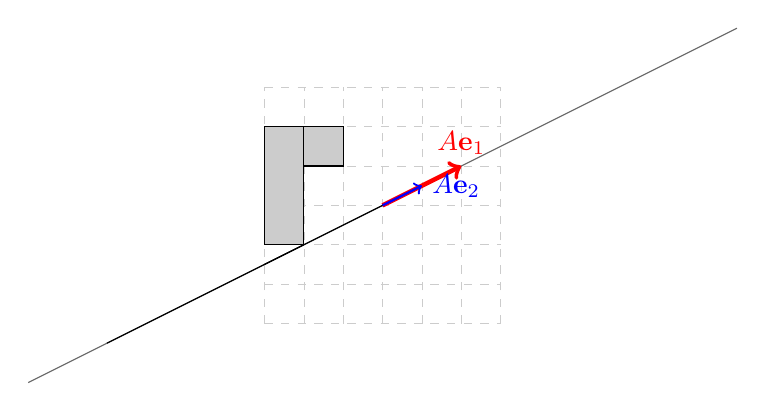
\begin{tikzpicture}[scale=.5]
    \draw [very thin,gray!40,dashed] (-3,-3) grid (3,3);
           \draw[fill=gray!40] (-3,-1) rectangle (-2,2);
       \draw[fill=gray!40] (-2,1) rectangle (-1,2);
    %Specify the transformation matrix and the center point
    \pgftransformcm{2}{1}{1}{.5}{\pgfpoint{0}{0}}
    \draw [black!60] (-3,-3) grid (3,3);
    \draw [ultra thick,red,->] (0,0)  -- (1,0) node [above] {$A\vec{e}_1$}; 
    \draw [thick,blue,->] (0,0) -- (0,1) node [right] {$A\vec{e}_2$};
        \draw[fill=black] (-3,-1) rectangle (-2,2);
     \draw[fill=black] (-2,1) rectangle (-1,2);
\end{tikzpicture}


\item \

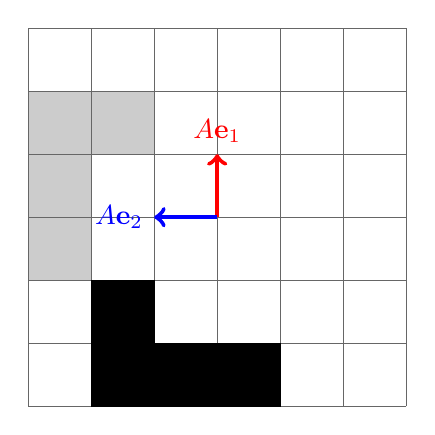
\begin{tikzpicture}[scale=.8]
    \draw [very thin,gray!40,dashed] (-3,-3) grid (3,3);
           \draw[fill=gray!40] (-3,-1) rectangle (-2,2);
       \draw[fill=gray!40] (-2,1) rectangle (-1,2);
    %Specify the transformation matrix and the center point
    \pgftransformcm{0}{1}{-1}{0}{\pgfpoint{0}{0}}
    \draw [black!60] (-3,-3) grid (3,3);
    \draw [ultra thick,red,->] (0,0)  -- (1,0) node [above] {$A\vec{e}_1$}; 
    \draw [ultra thick,blue,->] (0,0) -- (0,1) node [left] {$A\vec{e}_2$};
        \draw[fill=black] (-3,-1) rectangle (-2,2);
     \draw[fill=black] (-2,1) rectangle (-1,2);
\end{tikzpicture}

\item \

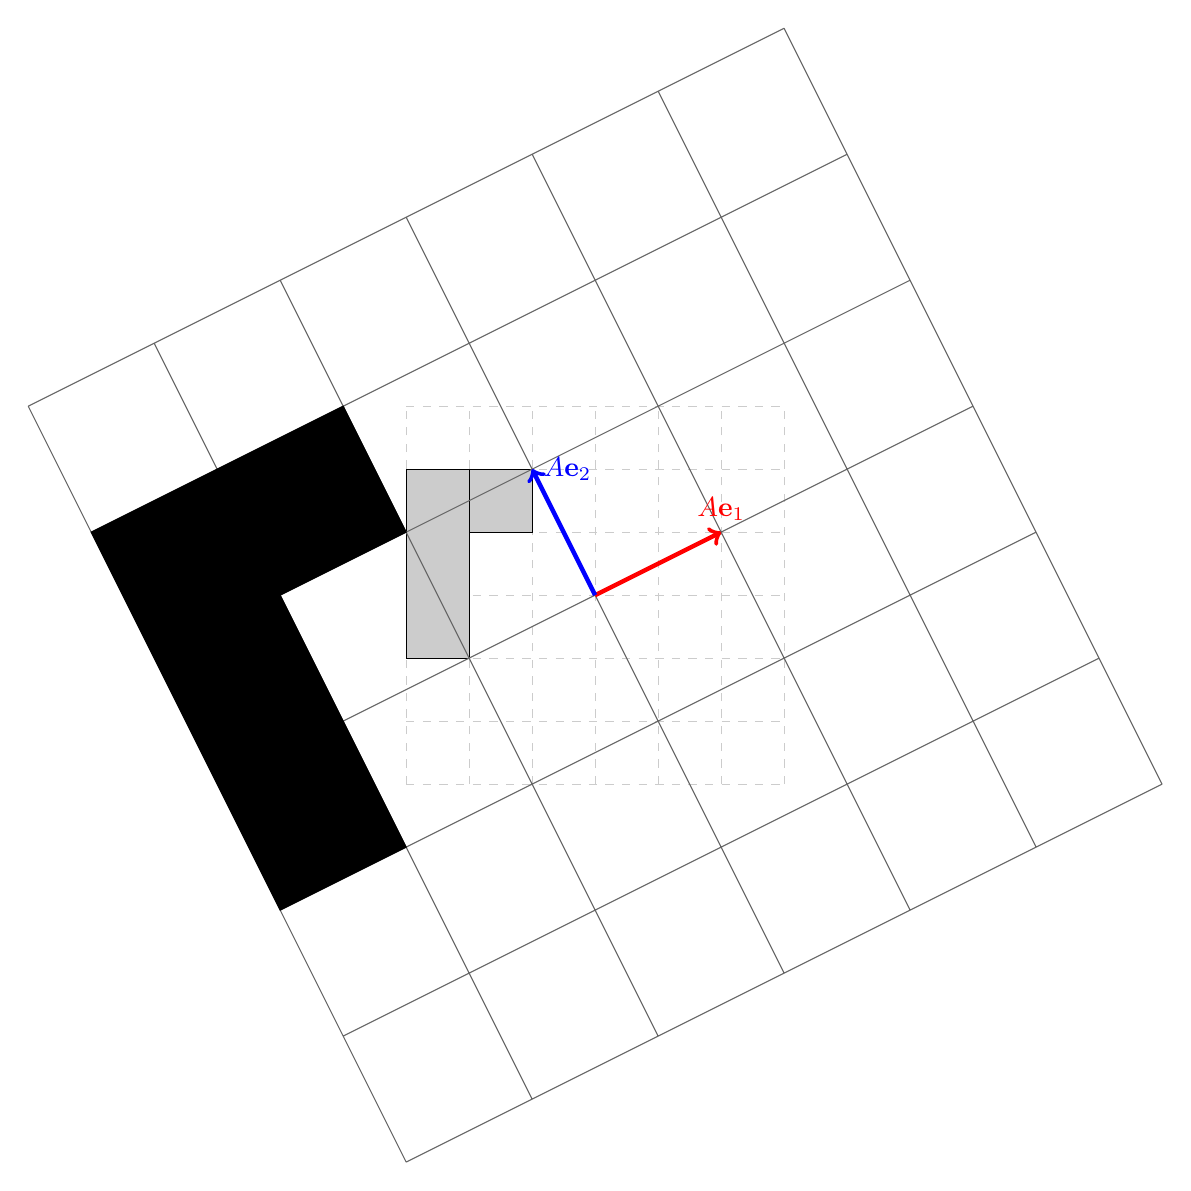
\begin{tikzpicture}[scale=.8]
    \draw [very thin,gray!40,dashed] (-3,-3) grid (3,3);
           \draw[fill=gray!40] (-3,-1) rectangle (-2,2);
       \draw[fill=gray!40] (-2,1) rectangle (-1,2);
    %Specify the transformation matrix and the center point
    \pgftransformcm{2}{1}{-1}{2}{\pgfpoint{0}{0}}
    \draw [black!60] (-3,-3) grid (3,3);
    \draw [ultra thick,red,->] (0,0)  -- (1,0) node [above] {$A\vec{e}_1$}; 
    \draw [ultra thick,blue,->] (0,0) -- (0,1) node [right] {$A\vec{e}_2$};
        \draw[fill=black] (-3,-1) rectangle (-2,2);
     \draw[fill=black] (-2,1) rectangle (-1,2);
\end{tikzpicture}


\item \

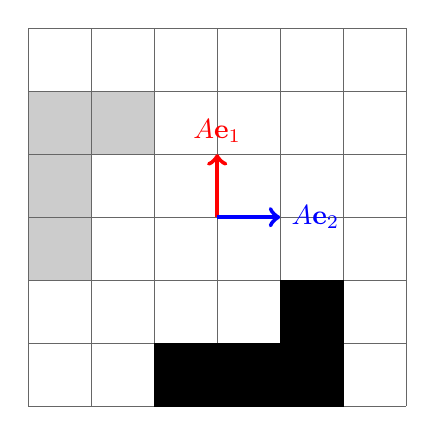
\begin{tikzpicture}[scale=.8]
    \draw [very thin,gray!40,dashed] (-3,-3) grid (3,3);
           \draw[fill=gray!40] (-3,-1) rectangle (-2,2);
       \draw[fill=gray!40] (-2,1) rectangle (-1,2);
    %Specify the transformation matrix and the center point
    \pgftransformcm{0}{1}{1}{0}{\pgfpoint{0}{0}}
    \draw [black!60] (-3,-3) grid (3,3);
    \draw [ultra thick,red,->] (0,0)  -- (1,0) node [above] {$A\vec{e}_1$}; 
    \draw [ultra thick,blue,->] (0,0) -- (0,1) node [right] {$A\vec{e}_2$};
        \draw[fill=black] (-3,-1) rectangle (-2,2);
     \draw[fill=black] (-2,1) rectangle (-1,2);
\end{tikzpicture}

\item \

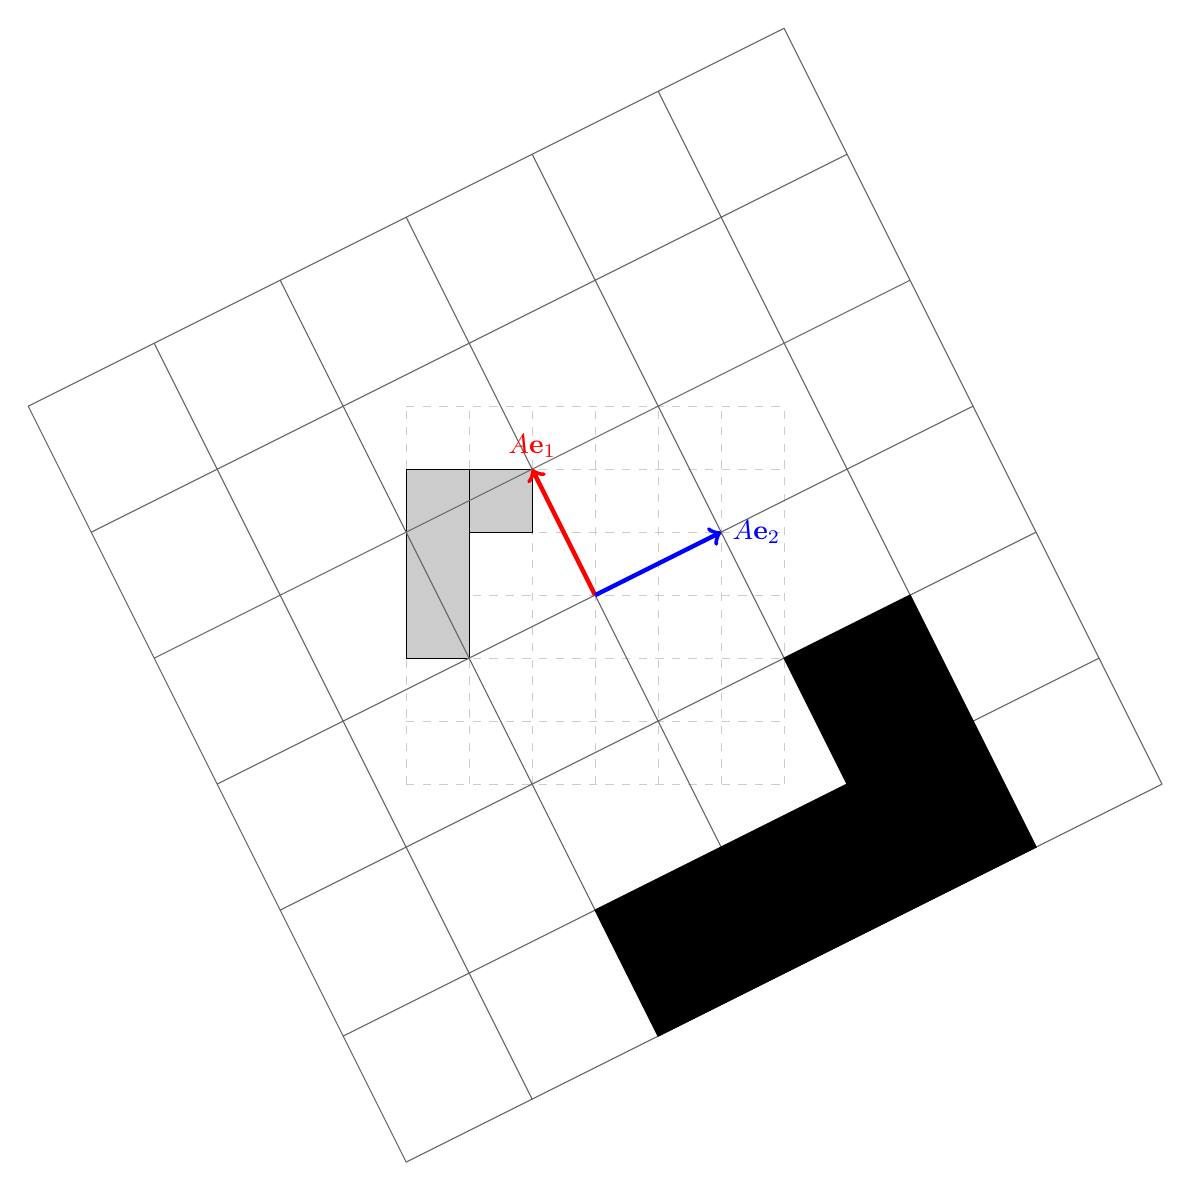
\begin{tikzpicture}[scale=.8]
    \draw [very thin,gray!40,dashed] (-3,-3) grid (3,3);
           \draw[fill=gray!40] (-3,-1) rectangle (-2,2);
       \draw[fill=gray!40] (-2,1) rectangle (-1,2);
    %Specify the transformation matrix and the center point
    \pgftransformcm{-1}{2}{2}{1}{\pgfpoint{0}{0}}
    \draw [black!60] (-3,-3) grid (3,3);
    \draw [ultra thick,red,->] (0,0)  -- (1,0) node [above] {$A\vec{e}_1$}; 
    \draw [ultra thick,blue,->] (0,0) -- (0,1) node [right] {$A\vec{e}_2$};
        \draw[fill=black] (-3,-1) rectangle (-2,2);
     \draw[fill=black] (-2,1) rectangle (-1,2);
\end{tikzpicture}


\end{enumerate}

 \begin{sol}
Write your solution here.
\end{sol}
\clearpage

\section*{Optional Problems}

\item Prove that any method for transforming a given permutation matrix $P$ to the identity matrix by row swaps will always do so with an even number of swaps or an odd number of swaps (depending on $P$).  In other words, while different methods of transforming $P$ to $I$ may take different numbers of swaps, the parity will be the same.

\item Using the notation for rotation and reflection matrices in Problem~\ref{rotref},
\begin{enumerate}
\item Verify that $R_\theta R_\phi = R_{\theta + \phi}$.
\item What type of transformation is $R_\theta r_\phi$?
\item What type of transformation is $r_\theta R_\phi$?
\item What type of transformation is $r_\theta r_\phi$?
\end{enumerate}

\item Prove that any orthogonal $2 \times 2$ matrix is either a rotation matrix or a reflection matrix.


\end{enumerate}




\end{document}